\chapter{Introduzione ad Ethereum}
Ethereum è un piattaforma di calcolo decentralizzata che permette di eseguire programmi
chiamati \textit{Smart Contracts},
sfruttando la blockchain per sincronizzare e salvare i cambiamenti di stato del sistema.
Spesso viene denotata con "World Computer".
Oltre ai contratti, ethereum sfrutta anche una criptovaluta chiamata \textit{Ether} per
misurare e vincolare le risorse per l'esecuzione dei contratti.


\begin{figure}[H]
      \centering
      
\includegraphics[width=1cm, keepaspectratio]{capitoli/ethereum/imgs/ethereum.png}
      \caption{Logo di Ethereum.}
\end{figure}

\section{Ethereum vs Bitcoin}
Per alcuni aspetti Ethereum può essere comparato a Bitcoin,
possiamo notare le seguenti caratteristiche comuni:

\begin{itemize}
      \item P2P,
      \item Un algoritmo di consenso per sincronizzare gli stati,
      \item Concetto simile alla PoW (Proof of Work),
      \item Utilizzo di funzioni crittografiche (hash, firme digitali, ...),
      \item Criptovaluta.
\end{itemize}

Tuttavia presenta anche molte differenze sostanziali:

\begin{itemize}
      \item Ethereum non è stato sviluppato per pagamenti, ma è una piattaforma di calcolo
            decentralizzata
      \item La criptovaluta è utilizzata solo come compenso per permettere
            l'utilizzo delle piattaforme di Ethereum
      \item Il linguaggio utilizzato da Ethereum è \textit{Turing-Completo} e dunque
            la blockchain può funzionare come un computer general purpose.
            Quello di Bitcoin è intenzionalmente limitato a valutazioni \verb|true/false|,
            non è quindi Turing-Completo e risulta molto più sicuro.
      \item La disponibilità massima di Bitcoin è pari a 21 milioni di unità, mentre gli
            Ether sono illimitati.
\end{itemize}

\section{Componenti della Blockchain}

Una blockchain pubblica è solitamente formata dai seguenti elementi:

\begin{itemize}
      \item \textbf{Una rete P2P}: serve per connettere i partecipanti e propagare le transazioni
      \item \textbf{Messaggi}: sono le transazioni
      \item \textbf{Regole del consenso}: dettano cosa costituisce una transazione valida
      \item \textbf{La Macchina degli stati}: calcola la transazione seguendo le regole del consenso
      \item \textbf{Una Catena di blocchi crittografati}: fungono da libro mastro per tutte
            le transazioni effettuate
      \item \textbf{Un algoritmo di consenso}: decentralizza il controllo della blockchain
      \item \textbf{Un sistema di incentivi}: ricompense date per chi approva le transazioni
            affinché queste ultime continuino ad essere approvate
      \item \textbf{Un Client}: implementazioni software dei precedenti punti
\end{itemize}

Nello specifico in Ethereum abbiamo:

\begin{itemize}
      \item \textbf{Rete P2P}: si chiama \textit{Ethereum Main Network} ed
            utilizza un protocollo chiamato \DH$\equiv$Vp2p.
      \item \textbf{Regole del Consenso}: sono definite in una specifica di riferimento chiamata
            Yellow Paper.
      \item \textbf{Transaction}: sono messaggi di rete che includono mittente, destinatario,
            valore, data payload, ...
      \item \textbf{State Machine}: le transizioni di stato di Ethereum sono processate dalla
            EVM (Ethereum Virtual Machine), una stack-based virtual machine che esegue il bytecode
            degli smart contracts. Questi vengono scritti in uno speciale linguaggio ad alto livello
            (come Solidity).
      \item \textbf{Data Structure}: lo stato di Ethereum è salvato localmente su ogni nodo come
            un database contenente transazioni e stato del sistema in una struttura dati chiamata
            \textit{Merker Patricia Tree}.
      \item \textbf{Algoritmo del Consenso}: Ethereum utilizza lo stesso metodo dei Bitcoin
            (Nakamoto Consensus) che utilizza la PoW per approvare le transazioni,
            determinando così lo stato attuale in base a qual'è la catena più lunga.
            Ci sono piani per passare alla PoS (Proof of Stake) che verranno introdotti dal
            progetto Casper.
      \item \textbf{Economic Security}: Ethereum utilizza un algoritmo di PoW chiamato \textit{Ethash},
            ma verrà abbandonato quando si passerà alla PoS.
      \item \textbf{Clients}: Ethereum ha diverse implementazioni di vari client,
            tutte quante valide ed intercambiabili, tra cui Go-Ethereum (Geth) e Parity.
\end{itemize}

\section{Implicazioni della Turing-Completezza}
Come sappiamo dall'Halting Problem, non possiamo a priori simulare un programma per
determinare se esso si arresterà oppure no. Poiché il linguaggio utilizzato da Ethereum è
Turing-Completo, gli smart contracts possono incappare in loop infiniti. Questo risulta
particolarmente problematico nelle blockchain pubbliche dato che non ci sarà modo di interromperli
(esempio della stampante). Per evitare questi problemi, che sono effettivamente degli attacchi DoS,
Ethereum introduce un meccanismo di misurazione chiamato \textbf{Gas}, in cui ogni operazione
effettuata dallo smart contract ha un costo in gas. Prima dell'esecuzione dello smart contract
viene imposto un limite massimo di gas utilizzabile per l'esecuzione del codice.
Dunque, se uno smart contract dovesse superare la soglia massima di gas consentitagli,
verrà interrotto.\\

Il gas si acquista con gli ether quando viene lanciato uno smart contract,
dunque si paga per un numero massimo di istruzioni che quello smart contract può eseguire.
Tutto il gas avanzato viene rimborsato al client sotto forma di ether.

\begin{figure}[H]
      \centering
      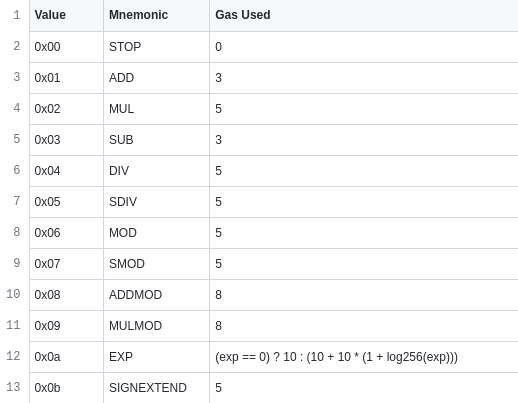
\includegraphics[width=10cm, keepaspectratio]{capitoli/ethereum/imgs/costo_gas.png}
      \caption{Costo in Gas di alcune operazioni.}
\end{figure}

\section{DApps}

Sono degli applicativi web, riconducibili a smart contracts, che vengono costruiti sopra
un'infrastruttura aperta, decentralizzata e P2P.
Sono composti sempre da:

\begin{itemize}
      \item uno smart contract
      \item alcune interfacce utenti web
\end{itemize}

Ma possono anche presentare:

\begin{itemize}
      \item Protocolli e piattaforme di memorizzazione decentralizzate
      \item Protocolli e piattaforme di comunicazione decentralizzate
\end{itemize}

\section{JSON-RPC}

Affinché un'applicazione software interagisca con la blockchain di Ethereum
(leggendo i dati della blockchain e/o inviando le transazioni alla rete), deve connettersi a
un nodo di Ethereum.
A tale scopo, ogni client di Ethereum implementa una specifica di JSON-RPC, in modo tale che vi
sia una serie uniforme di metodi su cui si basano le applicazioni.
JSON-RPC è un protocollo di chiamata della procedura remota (RPC) leggero e privo di stato.
Principalmente, la specifica definisce diverse strutture di dati e le regole intorno alla loro
elaborazione. È indipendente dal trasporto, poiché i concetti sono utilizzabili entro lo stesso
processo, su prese, via HTTP o in svariati ambienti di passaggio dei messaggi. Usa JSON (RFC 4627)
come formato dei dati.
Di solito, l'accesso alle RPC è fornito da un servizio HTTP sulla porta 8584 che
generalmente è accessibile solo da localhost.

\begin{lstlisting}[language=Bash, caption=Esempio di richiesta tramite jsonrpc]
$ curl -X POST \ 
       -H "Content-Type: application/json" \  
       --data \
       '{
           "jsonrpc":"2.0",
           "method":"eth_gasPrice",
           "params":[],
           "id":4213
        }' \
 http://localhost:8545/
 
{"jsonrpc":"2.0","id":4213,"result":"0x430e23400"}
\end{lstlisting}

\section{Tipi di Account}

In Ethereum ci sono 2 tipologie di Account: EOA e Contracts Account.

\paragraph{Externally Owned Accounts (EOA):}
sono account che hanno una chiave privata e sono gestiti da una persona fisica.
Sono in grado di trasmettere e ricevere ether.

\paragraph{Contracts Accout:}
Questo tipo di account ha uno smart contract code che un semplice account esterno non può avere.
Non ha una chiave privata ed è posseduto e gestito dalla logica del suo smart contract.
Ha un suo indirizzo, e dunque può ricevere e mandare ether.
Quando esso è destinatario di una transazione, l'account eseguirà il codice del contratto
nella EVM utilizzando la transazione ed i dati presenti in essa come input.
Inoltre, può ricevere in input una transazione senza ether ma con dati ed una specifica
funzione del suo codice da eseguire. Questo tipo di account, non avendo una chiave privata
non può iniziare transazioni, ma può solo reagire a transazioni chiamando altri contratti o
spostando ether.

\section{Proof of Stake (PoS)}
Come il PoW, il PoS (Proof of Stake) è un modo per validare e dare consenso alle
transazioni. Il PoW paga miner che risolvono problemi matematici con lo scopo di
creare e validare nuovi blocchi per far crescere la blockchain.
Con il PoS, il creatore  di un nuovo blocco viene scelto in base alla quantità
di moneta che possiede, quanto "stake" ha quella persona nella determinata moneta
(currency). \textit{More stake, more power}.
Lo stake non è solo definito come la quantità di moneta posseduta ma è importante
anche da quanto tempo questa persona possiede la valuta.
Per esempio, se una persona ha comprato recentemente una grossa somma di
cryptocurrency, il suo stake sarà inferiore a quello di una persona che possiede
meno moneta ma da molto più tempo.
Questo sistema scoraggia gli hacker in quanto per dominare la blockchain è
necessario avere tanto stake e possederlo da molto tempo.
Il principale vantaggio di questo sistema è il risparmio energetico,
non servono immense potenze di calcolo per risolvere complesse operazioni matematiche.
Alcune cryptocurrencies che sfruttano il PoS sono:

\begin{itemize}
      \item ShadowCash
      \item Nxt
      \item BlockCoin
      \item Nav Coin
\end{itemize}

\section{Smart Contracts}

Il termine Smart Contract è stato coniato da Nick Szabo ed è definito come:
"un insieme di promesse, specificato in forma digitale che includono protocolli,
all'interno dei quali le due parti coinvolte adempiono alle loro promesse
contrattuali".
Il concetto di Smart Contract quando usato in riferimento ad Ethereum può essere
fuorviante in quanto
non si riferisce a contratti legali ma ad un programma software che viene eseguito
dalla EVM sull'Ethereum
World Computer. Gli Smart Contract hanno 2 caratteristiche:

\begin{itemize}
      \item Sono \textbf{immutabili}: una volta mandato in esecuzione il
            codice di uno smart contract esso non potrà cambiare.
            L'unico modo per modificarne il codice è quello di effettuare un
            nuovo deployment.
      \item Sono \textbf{deterministici}: l'output di uno smart contract sarà
            sempre lo stesso su ogni macchina che lo esegue dato il contesto della
            transazione che lo ha inizializzato e lo stato della blockchain nel momento
            dell'esecuzione.
\end{itemize}

\section{Coins and Tokens}
In questo paragrafo andremo ad analizzare brevemente le differenze tra Coin e Token.

\paragraph{Coins:}
un Coin può essere definito tale se rispetta le seguenti caratteristiche:

\begin{enumerate}
      \item Opera all'interno della sua blockchain
      \item Funziona come denaro
      \item Può essere minato
\end{enumerate}

\paragraph{Tokens:}
la principale differenza con i Coin è che un Token non ha una sua propria blockchain
ma si appoggia ad altre già esistenti, come per esempio ERC20, BAT e BNT che
sfruttano Ethereum. Un'altra sostanziale differenza è che le transazioni di Coins
sono gestite dalla blockchain mentre quelle di token sono governate da Smart Contract.
Quando un token viene "speso" viene fisicamente spostato da un posto ad un altro,
a differenza dei Coin, quando un coin viene speso viene solo aggiornato il saldo
delle due parti. Un esempio di token sono gli NFT (Non Fungible Tokens).

\section{Hard Fork}

\paragraph{Block \#1,192,000} \ \\
DAO - Un Hard Fork che rimborsò le vittime dell'attacco al contratto DAO e causò
la separazione tra Ethereum ed Ethereum Classic.

\paragraph{Block \#2,463,000} \ \\
Tangerine Whistle — Un Hard Fok avvenuto per cambiare il costo in gas di certe
operazioni di I/O e per risanare lo stato della blockchain da alcuni attacchi
DoS che sfruttavano queste operazioni a bassissimo costo.

\paragraph{Block \#2,675,000} \ \\
Spurious Dragon — Un Hard Fork che introdusse protezione ad altre forme di DoS
e aggiunse un nuovo meccanismo di protezione a replay attack.